%\begin{filecontents*}[noheader,force]{sample1.m4}

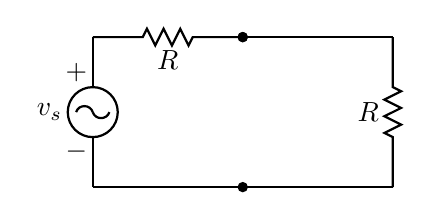
\begin{tikzpicture}[scale=2.54]
% dpic version 2014.Jan.01 option -g for TikZ and PGF 1.01
\ifx\dpiclw\undefined\newdimen\dpiclw\fi
\global\def\dpicdraw{\draw[line width=\dpiclw]}
\global\def\dpicstop{;}
\dpiclw=0.8bp
\dpiclw=0.8bp
\dpicdraw (0,0)
 --(0,0.25)\dpicstop
\dpicdraw (0,0.375) circle (0.049213in)\dpicstop
\dpicdraw (-0,0.375)
 ..controls (-0.013347,0.415042) and (-0.069986,0.415042)
 ..(-0.083333,0.375)\dpicstop
\dpicdraw (0,0.375)
 ..controls (0.013347,0.334958) and (0.069986,0.334958)
 ..(0.083333,0.375)\dpicstop
\dpicdraw (0,0.5)
 --(0,0.75)\dpicstop
\draw (0,0.25) node[below left=-1.5bp]{$ -$};
\draw (-0.125,0.375) node[left=-1.5bp]{$ v_s$};
\draw (0,0.5) node[above left=-1.5bp]{$ +$};
\dpicdraw (0,0.75)
 --(0.25,0.75)
 --(0.270833,0.791667)
 --(0.3125,0.708333)
 --(0.354167,0.791667)
 --(0.395833,0.708333)
 --(0.4375,0.791667)
 --(0.479167,0.708333)
 --(0.5,0.75)
 --(0.75,0.75)\dpicstop
\draw (0.375,0.708333) node[below=-1.5bp]{$ R$};
\dpicdraw[fill=black](0.75,0.75) circle (0.007874in)\dpicstop
\dpicdraw[fill=black](0.75,0.75) circle (0.007874in)\dpicstop
\dpicdraw (0.75,0.75)
 --(1.5,0.75)\dpicstop
\dpicdraw (1.5,0.75)
 --(1.5,0.5)
 --(1.541667,0.479167)
 --(1.458333,0.4375)
 --(1.541667,0.395833)
 --(1.458333,0.354167)
 --(1.541667,0.3125)
 --(1.458333,0.270833)
 --(1.5,0.25)
 --(1.5,0)\dpicstop
\draw (1.458333,0.375) node[left=-1.5bp]{$ R$};
\dpicdraw (1.5,0)
 --(0.75,0)\dpicstop
\dpicdraw[fill=black](0.75,0) circle (0.007874in)\dpicstop
\dpicdraw (0.75,0)
 --(0,0)\dpicstop
\end{tikzpicture}
